\documentclass[11pt]{scrartcl}
%%
%
% This is a poster template with latex macros and using
% the University of Florida Logo.  For further information
% on making postscript, resizeing, and printing the poster file
% please see web site 
% http://www.phys.ufl.edu/~pjh/posters/poster_howto.html
% 
% N.B. This format is cribbed from one obtained from the University
% of Karlsruhe, so some macro names and parameters are in German
% Here is a short glosary:
% Breite: width
% Hoehe: height
% sPALTE: column
% Kasten: box
%
% All style files necessary are part of standard TeTeX distribution
% On the UF unix cluster you should not need to import these files
% specially, as they will be automatically located.  If you
% run on a local PC however, you will need to locate these files.
% At UF try /usr/local/TeTeX...
% 
% P. Hirschfeld 2/11/00
%
% The recommended procedure is to first generate a ``Special Format" size poster
% file, which is relatively easy to manipulate and view.  It can be
% resized later to A0 (900 x 1100 mm) full poster size, or A4 or Letter size
% as desired (see web site).  Note the large format printers currently
% in use at UF's OIR have max width of about 90cm or 3 ft., but the paper
% comes in rolls so the length is variable.  See below the specifications
% for width and height of various formats.  Default in the template is
% ``Special Format",  with 4 columns.
%%
%% 
%% Choose your poster size:
%% For printing you will later RESIZE your poster by a factor
%%        2*sqrt(2) = 2.828    (for A0)
%%        2         = 2.00     (for A1) 
%%  
%% 
\def\breite{400mm}     % Special Format. 
\def\hoehe{400mm}      % Scaled by 2.82 this gives 110cm x 90cm 

%\def\breite{390mm}     % Special Format. 
%\def\hoehe{319.2mm}      % Scaled by 2.82 this gives 110cm x 90cm 
\def\anzspalten{2}
%%
%%\def\breite{420mm}     % A3 LANDSCAPE
%%\def\hoehe{297mm}
%%\def\anzspalten{4}
%%
%% \def\breite{297mm}     % A3 PORTRAIT
%% \def\hoehe{420mm}
%% \def\anzspalten{3}
%%
%% \def\breite{210mm}     % A4 PORTRAIT
%% \def\hoehe{297mm}
%% \def\anzspalten{2}
%%
%%
%% Procedure:
%%   Generate poster.dvi with latex
%%   Check with Ghostview
%%   Make a .ps-file with ``dvips -o poster.ps poster''
%%   Scale it with poster_resize poster.ps S
%%   where S is scale factor
%%     for Special Format->A0 S= 2.828 (= 2^(3/2)))
%%     for Special Format->A1 S= 2 (= 2^(2/2)))
%% 
%% Sizes (European:)
%%   A3: 29.73 X 42.04 cm
%%   A1: 59.5 X 84.1 cm
%%   A0: 84.1 X 118.9 cm
%%   N.B. The recommended procedure is ``Special Format x 2.82"
%%   which gives 90cm x 110cm (not quite A0 dimensions).
%%
%% --------------------------------------------------------------------------
%%
%% Load the necessary packages
%% 
\usepackage{palatino}
\usepackage[latin1]{inputenc}
\usepackage{epsf}
\usepackage{graphicx,psfrag,color,pstricks,pst-grad}
\usepackage{amsmath,amssymb}
\usepackage{latexsym}
\usepackage{calc}
\usepackage{multicol}
\usepackage{url}
%%
%% Define the required numbers, lengths and boxes 
%%
\newsavebox{\dummybox}
\newsavebox{\spalten}
%\input psfig.sty

%%
%%
\newlength{\bgwidth}\newlength{\bgheight}
\setlength\bgheight{\hoehe} \addtolength\bgheight{-1mm}
\setlength\bgwidth{\breite} \addtolength\bgwidth{-1mm}

\newlength{\kastenwidth}

%% Set paper format
\setlength\paperheight{\hoehe}                                             
\setlength\paperwidth{\breite}
\special{papersize=\breite,\hoehe}

\topmargin -1in
\marginparsep0mm
\marginparwidth0mm
\headheight0mm
\headsep0mm


%% Minimal Margins to Make Correct Bounding Box
%\setlength{\oddsidemargin}{-2.44cm}
%\addtolength{\topmargin}{-3mm}
\setlength{\oddsidemargin}{-2.44cm}
\addtolength{\topmargin}{-3mm}
\textwidth\paperwidth
\textheight\paperheight

%%
%%
\parindent0cm
\parskip1.5ex plus0.5ex minus 0.5ex
\pagestyle{empty}




\definecolor{recoilcolor}{rgb}{1,0,0}
\definecolor{occolor}{rgb}{0,1,0}
\definecolor{pink}{rgb}{0,1,1}





\def\UberStil{\normalfont\sffamily\bfseries\large}
\def\UnterStil{\normalfont\sffamily\small}
\def\LabelStil{\normalfont\sffamily\tiny}
\def\LegStil{\normalfont\sffamily\tiny}

%%
%% Define some commands
%%
\definecolor{JG}{rgb}{0.1,0.9,0.3}

\newenvironment{kasten}{
  \begin{lrbox}{\dummybox}
    \begin{minipage}{\linewidth}}
    {\end{minipage}
  \end{lrbox}
  \raisebox{-\depth}{\psshadowbox[cornersize=absolute,linearc=14pt,framesep=1em]{\usebox{\dummybox}}}\\[0.5em]}
\newenvironment{spalte}{
  \setlength\kastenwidth{1.2\textwidth}
  \divide\kastenwidth by \anzspalten
  \begin{minipage}[t]{\kastenwidth}}{\end{minipage}}

%\renewcommand{\emph}[1]{{\color{red}\textbf{#1}}}


%\def\op#1{\hat{#1}}
\begin{document}
%%%%%%%%%%%%%%%%%%%%%%%%%%%%%%%%%%%%%%%%%%%%%%%%%%%%
%%%               Background                     %%%
%%%%%%%%%%%%%%%%%%%%%%%%%%%%%%%%%%%%%%%%%%%%%%%%%%%%
{\newrgbcolor{gradbegin}{0.5 0.5 1}
  \newrgbcolor{gradend}{1 1 1}%{1 1 0.5}%
  %\rput[cm](15.23,-15){
  \rput[tl]{0}(0,0){
  \includegraphics[width=\paperwidth]{logos/antenna1} %lower resolution
  %\includegraphics[width=\paperwidth]{logos/alma_logo} %higher resolution
  }
\vfill}

%{\newrgbcolor{gradbegin}{0.5 0.5 1}%
%  \newrgbcolor{gradend}{1 1 1}%{1 1 0.5}%
%  \psframe[fillstyle=gradient,gradend=gradend,%
%  gradbegin=gradbegin,gradmidpoint=0.1](\bgwidth,-\bgheight)}
%\vfill
%%%%%%%%%%%%%%%%%%%%%%%%%%%%%%%%%%%%%%%%%%%%%%%%%%%%
%%%                     Header                   %%%
%%%%%%%%%%%%%%%%%%%%%%%%%%%%%%%%%%%%%%%%%%%%%%%%%%%%
\hfill
\psshadowbox{\makebox[0.95\textwidth]{%
    \hfill
	\parbox[c]{2cm}{\includegraphics[width=2cm,height=!]{logos/alma_logo}}
    \hfill
    \parbox[c]{0.7\linewidth}{%
      \begin{center}
		\textbf{\Huge {High Performance Graphical Data Trending in a Distributed System}}\\[0.5em]
		\textsc{\large Cristi\'{a}n Maureira$^{1}$, Arturo Hoffstadt$^{1}$,
		Joao L\'{o}pez$^{1}$, Nicol\'{a}s Troncoso$^{2}$, Rodrigo Tobar$^{3}$,
		Horst H. von Brand$^{1}$\\[0.3em]
		{ $^1$Computer Systems Research Group, Universidad T\'ecnica
		Federico Santa Mar\'ia (UTFSM), Valpara\'iso, Chile}\\
		{ $^2$Associated Universities, Inc. (AUI), Santiago, Chile;
		Universidad T\'ecnica Federico Santa Mar\'ia, Valpara\'{i}so, Chile}\\
		{ $^3$European Southern Observatory (ESO), Garching bei M\"{u}nchen, Germany}}
      \end{center}}
	\hfill
    \parbox[c]{2cm}{\includegraphics[width=3cm,height=!]{logos/usm_logo}}
	\hfill
\hfill}}\hfill\mbox{}\\

\hfill
\psshadowbox{\makebox[0.83\textwidth]{%
    \hfill
    \parbox[t]{0.8\linewidth}{%
\hfill{\large\bf{\color{red}ABSTRACT}}\hfill\mbox{}\\
Trending near real-time data is a complex task, specially in distributed environments. This problem was typically tackled in financial and transaction systems, but now it applies to its out-most in hardware monitoring of radio-antenna arrays. Data handling requires subscription to specific data feeds that needs to be implemented avoiding replication, and data rate of transmission has to be assured. On the side of the graphical client, rendering needs to be fast enough so it may be perceived as real-time processing and display.\\\vspace{-0.1cm}

In this context the ALMA Common Software (ACS)[1] provides a software
infrastructure for distributed projects, which may require trending large
volumes of data. For this requirements, ACS offers a Sampling System, which
allows sampling selected data feed in different frequencies, reason to develop
an application with good trending performance. Currently there are many
graphical libraries available for data trending. This imposes a problem when
trying to choose a library: it is necessary to know which one has the best
performance, and which combination with a programming language is the best
decision.\\\vspace{-0.1cm}

This work presents a performance study of different graphical libraries and languages in order to present the optimal environment when writing or re-factoring an application using trending technologies in distributed systems. To properly address the complexity at hand, a specific set of alternative was pre-selected, including libraries in Java and Python, languages which are part of ACS. The stress benchmark will be developed in a simulated distributed environment using ACS in order to test the trending libraries.
}
\hfill}}\hfill\mbox{}

\begin{lrbox}{\spalten}
  \parbox[t][0.61\textheight]{1.3\textwidth}{
   % \vspace*{0.2cm}
%%%%%%%%%%%%%%%%%%%%%%%%%%%%%%%%%%%%%%%%%%%%%%%%%%%%
%%%                 first column                 %%%             
%%%%%%%%%%%%%%%%%%%%%%%%%%%%%%%%%%%%%%%%%%%%%%%%%%%%
    \begin{spalte}
     
	  \begin{kasten}
        \section*{\hspace{0.2cm} {\color{red} Problem} }
			\begin{minipage}[t]{0.95\linewidth}
			When a development team is given the task of creating a software project,
			one of the first questions is the selection of the programming language.
			This is a very important decision, as performance is greatly affected by the
			paradigm and implementation of the available compilers for that programming
			language. The usual manner to solve this is to prototype, use previous
			experience and test the different wanted characteristics, such as
			modularity, performance, and scalability.
			
			%There are comparisons between different programming
			%languages, such as~\cite{empirical}, in which the author gives a walk
			%through the origin of each language, and puts emphasis in the validation
			%of a programming language comparison, because that depends on different
			%characteristics, such as programmer capabilities, the different task
			%and work conditions, the handling of misunderstood requirements,
			%the paradigms employed (object oriented, imperative, generic programming).
			%As is to be expected, such comparisons tend to concentrate only on one area.

			Aside the selection of programming language [2], the team has to
			consider the selection of a graphical library. This is a nested decision, as very
			few libraries are available for several languages.
			Then, the question arises: ``Of all the graphical libraries available, which is
			the best one for my project?''
			%Strictly speaking, one should analyse a couple of libraries and
			%then make a decision. In practice this is almost never done, as schedules are usually tight so
			%there is no time available to evaluate every choice.
			
			In our case, the main problem is to find the best choice in the data trending
			area, where performance of the graphical representation are critical.
			There are several ways to measure the performance and quality of graphical
			libraries, some examples are:\\

			\begin{minipage}[t]{0.3\linewidth}
			\begin{itemize}
			    \item Number of chart types handled.
			    \item Trace options.
			\end{itemize}
			\end{minipage}
			\begin{minipage}[t]{0.3\linewidth}
			\begin{itemize}
			    \item Plot functionality.
			    \item Frames Per Second (FPS).
			\end{itemize}
			\end{minipage}
			\begin{minipage}[t]{0.3\linewidth}
			\begin{itemize}
		        \item Data volume vs. performance
			\end{itemize}
			\end{minipage}
			\\

			In the present work the most important metrics are FPS and the data
			volume vs. performance. Large amounts of data need to be quickly processed
			and displayed, together with additional information.
			
			%The development team has still two decisions open, both of them pending from a
			%proper comparison. But there is yet another problem.
			%Many systems in real world applications are not \emph{single-node} systems,
			%so that performance tested on a single computer may give a different result
			%%than when deployed on a distributed system. This is the case of
			%%ALMA and ALMA Common Software (ACS) distributed applications. Distributed systems are complex, and
			%%communications is an important part of the data pre-processing.
			
			Given this, a third question remains open: ``How does a distributed system
			affect my trending application's performance?''			
		\end{minipage} \hfill
      \end{kasten}
	  \begin{kasten}
        \section*{\hspace{0.2cm} {\color{red} Real Benchmark} }
			\vspace{-0.1cm}
			\begin{minipage}[t]{0.43\linewidth}
			This section presents the result of testing the Sampling System GUI[3] in a real case scenario at the ALMA Observatory.
			The Sampling System GUI is used in the same deployment as the operations software (ALMASW).
			This Figure roughly shows the distributed environment where ALMASW and the Sampling System GUI are deployed.

			ACS and the sampling system[4] run on the ACS server. The sampling system GUI is run from the operations console.
			This setup was selected to monitor the behavior of the FrontEnd receiver during its locking routine.
			The monitoring setup considered two charts, each with:
			\begin{itemize}
				\item Five properties being sampled.
				\item Sampling frequency of 20\,[Hz].
				\item Store a window of 15 minutes of plots.
				\item Storing all of the data to disk.
			\end{itemize}
			\end{minipage} \hspace{0.4cm} %\hfill
			\begin{minipage}[t]{0.50\linewidth}
			\strut\vskip -\baselineskip
			\hfill
			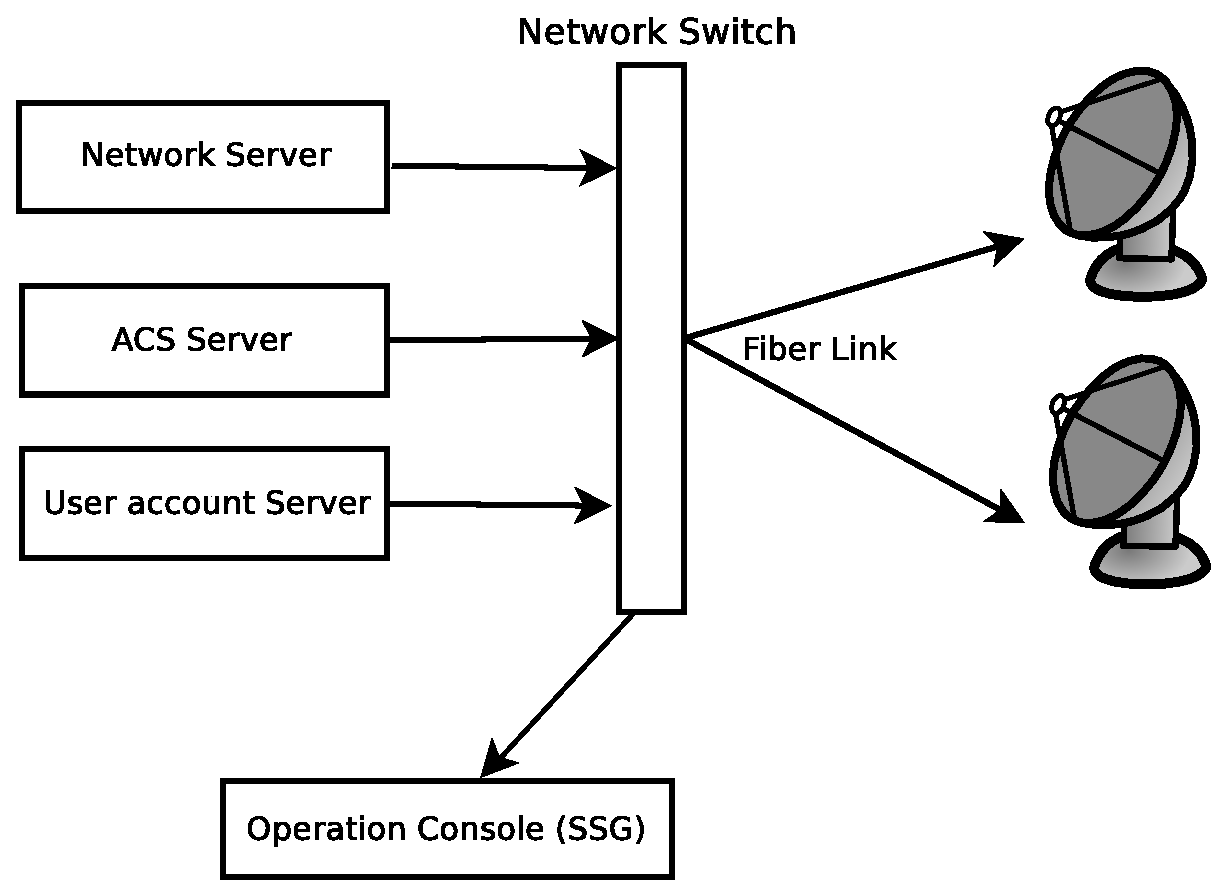
\includegraphics[width=1.0\linewidth]{../img/deployment}
			\vspace{0.1cm}
			\end{minipage}\vfill
			\vspace{-0.5cm}
			\begin{minipage}[t]{0.95\linewidth}
			20\,[Hz] is the maximum monitoring frequency available in ALMA since it is limited by its 48\,[ms] period.
			
			The test that was run on the FrontEnd receiver consisted in locking the band in 0.5\,[GHz] steps over the range of
			the four available bands. The test took approximately 4 hours, time during which the sampling system GUI was
			continuously plotting and saving data to disk. At the time of the test only two antennas were available,
			this test should be run again when there are six available antennas for such purpose. This would demonstrate how the
			overall system behaves when increasing the number of distributed nodes.
			
			The overall result of the Sampling System is positive, since it met all the engineering requirements for
			monitoring during the specified test. It could cope with the amount of properties and the sampling rates
			specified by the engineering division. Data was properly stored to disk, and the plots
			provided a quick look for the data before it was more thoroughly analyzed.
			\end{minipage}
	  \end{kasten}
    \end{spalte}
	 \hfill
%%%%%%%%%%%%%%%%%%%%%%%%%%%%%%%%%%%%%%%%%%%%%%%%%%%%
%%%               second column                  %%%             
%%%%%%%%%%%%%%%%%%%%%%%%%%%%%%%%%%%%%%%%%%%%%%%%%%%%
    \begin{spalte}
       
      \begin{kasten}
        \section*{\hspace{0.2cm} {\color{blue} Graphical Library Benchmark} }

			\begin{minipage}[t]{0.95\linewidth}
					Programming language and graphical library decissions
					are covered in a simple bnechmark conducted during research. The main purpose
					is to determine the fasted trending library. In ACS there are three available
					language for programming, which are C++, Java and Python. Among the available
					libraries, the research team selected the two most promissing (according to
					perceived performance and previous experience) and compared them. Each ``Set of
					data'' consists in 200 pair ($x,y$) of values to plot. FPS was
					measured for each of them, until a total of 2000 pairs. Speed indicates the
					rate at which data was fed to the program by the helper thread.
					
					% Comparisons were conducted using similar code structure: a thread to handle
					% random data feed, another thread handle program execution and trending. The
					%GUI  is as simple as possible, containing only the dynamic plotted data. The
					% platform in which the tests where conducted is an Intel (R) Core(TM)2 Duo 2.66
					% $[GHz]$, whit 4 GB Ram and Linux Fedora 12 x86. Important to note that NVIDIA
					% proprietary drivers were used.
			\end{minipage} \vspace{0.25cm}

			\begin{minipage}[t]{0.95\linewidth}
				\begin{center}
				% 100\,[ms] period
				\includegraphics[width=0.30\linewidth, height=!]{../img/java-100}
				% 10\,[ms] period
				\includegraphics[width=0.30\linewidth, height=!]{../img/java-10}
				% 1\,[ms] period
				\includegraphics[width=0.30\linewidth, height=!]{../img/java-1}\\
				Java libraries comparisons: JChart2D[5] and JFreeChart.
				\end{center}
			\end{minipage}

			\begin{minipage}[t]{0.95\linewidth}
				\begin{center}
				% 100\,[ms] period
				\includegraphics[width=0.30\linewidth, height=!]{../img/python-100}
				% 10\,[ms] period
				\includegraphics[width=0.30\linewidth, height=!]{../img/python-10}
				% 1\,[ms] period
				\includegraphics[width=0.30\linewidth, height=!]{../img/python-1}\\
				Python libraries comparisons: PyQwt and Matplotlib[8].
				\end{center}
			\end{minipage}

			\begin{minipage}[t]{0.95\linewidth}
				\begin{center}
				% 100\,[ms] period
				\includegraphics[width=0.30\linewidth, height=!]{../img/c++-100}
				% 10\,[ms] period
				\includegraphics[width=0.30\linewidth, height=!]{../img/c++-10}
				% 1\,[ms] period
				\includegraphics[width=0.30\linewidth, height=!]{../img/c++-1}\\
				C++ libraries comparisson: Qwt[9] and wxMathPlot.
				\end{center}
			\end{minipage} \vspace{0.45cm}

			\begin{minipage}[t]{0.95\linewidth}
JChart2D shows better and more stable performance tha JFreeChart. It is
important to notice the start-up time in Java language. In Python, PyQwt shows
greater performance than Mathplotlib, which is oriented for offline plotting.
In C++ FPS achieved increses dramatically, even then, Qwt has greater
performance than wxMathPlot. Is important to notice that for trending purposes
FPS in the range of 4 to 20 are commonly used. Less than this values creates
the perception of loss of internal locus, while greater than this is used in
real-time plotting.
			\end{minipage}
      \end{kasten}

    \end{spalte}
     \hfill\mbox{}
}

\end{lrbox}
\hfill
\resizebox*{0.95\textwidth}{!}{
  \usebox{\spalten}}\hfill\mbox{}

\vspace{0.1cm}
\hspace{1cm}
\psshadowbox[cornersize=absolute,linearc=14pt]{\makebox[0.923\textwidth]{%
 \hfill
 \parbox[t]{0.9\linewidth}{
\begin{minipage}[t]{0.95\linewidth}
\section*{ {\normalsize \color{red} Conclusions}}

{\footnotesize
%\renewcommand{\baselinestretch}{0.5}
			\begin{minipage}[t]{0.50\linewidth}
%			\begin{minipage}[t]{0.95\linewidth}
Better ways of measuring performance,
like the number of data streams that can be displayed at a given FPS
or the impact of smoothly evolving data or scattered points,
should be considered.

%Looking backwards, the evolution of the different libraries give the
%programmers a lot of ``path to follow'' when starting a new project.
%The performance
%of the actual data trending libraries in different languages is very important
%because all of them try to offer ``simple programming'' in this application
%area.
%Comparing the features of the libraries is not so important, because most of
%them
%are rather robust, and those with more features just allow creating more
%elaborate plots.
%Without going further, there are other characteristics to consider, like
%``perdurability,'' ``modularity,'' and ``scalability'' of software.
For a long-lived project like ALMA (and its supporting software ACS)
these characteristics are crucial.
How to estimate the stability and longer range development and maintenance
of open source software on which something like ACS is based is still very much
an open question.

Also, other important characteristics haven't been considered in detail.
For a long-lived protect like ALMA (and its supporting ACS package) using
stable, well-maintained base software is crucial.

			\end{minipage} \hspace{0.2cm}
			\begin{minipage}[t]{0.50\linewidth}

%In the Graphical Benchmark section we saw benchmarks of a couple of graphic
%libraries
%in the three languages that ACS uses, C++, Java, and Python.
The Graphical Benchmark shows the behaviour of these libraries in three levels
of stressed environments, giving us data to discriminate among them.
Anyway, this is not a final decision, because one benchmark is not enough to
test the real
performance of a graphical library, but it is a good start to help
discriminating them with the previous
basic functionality (plotting random data).

Finally, in the real benchmark section we can see the performance of
the existing scientific data visualization tool, developed by the Computer Systems Research Group (CSRG),
and giving us the chance to analyze a real application in a real distributed system such as the
ALMA project.
			\end{minipage}

}
\end{minipage}
}\hfill
}}\hfill\mbox{}\\
\vfill

\hfill
\psshadowbox{\makebox[0.922\linewidth]{
\hfill
\begin{minipage}[t]{0.30\linewidth}
	{\scriptsize
	{\small\bf Acknowledgements}
	
	\renewcommand{\baselinestretch}{0.5}
	This work and the associated research has been conducted with funds granted by
	CONICYT, specifically ALMA-CONICYT grant \#31090034 and \#31080031.
	Horst H. von Brand's work was also supported in part
	by Centro Cient\'\i fico-Tecnol\'ogico de Valpara\'\i so (CCTVal) grant FB0821.
	}
\end{minipage}\hfill

\begin{minipage}[t]{0.60\linewidth}
	{\scriptsize
	\renewcommand{\baselinestretch}{1.0}
	{\small\bf References}
	
	%[1] Brooks, M. et~al., ``ALMA Monitor and Control Bus Interface Specification''
	%in [{\em ALMA Documentation}{\hspace{0.1em}}], (2007).
	%\renewcommand{\baselinestretch}{0.5}
	[1] Chiozzi, G. et al., ``The ALMA Common Software: A developer friendly CORBA-based framework,'' in [Proceedings of SPIE 2004 ], (2004).
	\renewcommand{\baselinestretch}{0.5}
	
	[2] Prechelet, L., ``An empirical comparision of seven programming languages,'' Computer 33(10), 23-29 (2000)
	\renewcommand{\baselinestretch}{0.5}
	
	[3] Sampling System GUI Project \url{http://csrg.inf.utfsm.cl/twiki4/bin/view/ACS/SamplingSystem}
	\renewcommand{\baselinestretch}{0.5}
	
	[4] Marcantonio, P. D. et al., ``ACS sampling system: Design, implementation and performance evaluation,'' in [Proceedings of SPIE ], (2004).
	\renewcommand{\baselinestretch}{0.5}
	
	[5] Westermann, A., ``JChart2D.'' \url{http://jchart2d.sourceforge.net/index.shtml}.
	\renewcommand{\baselinestretch}{0.5}
%	}	
%\end{minipage}
%\begin{minipage}[t]{0.45\linewidth}
%	{\scriptsize
%	\renewcommand{\baselinestretch}{1.0}
%	\vspace{0.2cm}

	[6] Hunter, J. D., ``Matplotlib: A 2D graphics environment,'' Computing in Science \& Engineering 9(3), 90-95 (2007).
	\renewcommand{\baselinestretch}{0.5}
	
	[7] Rathmann, U. and Wilgen, J., ``Qwt - Qt widgets for technical applications.'' \url{http://qwt.sourceforge.net}.
	\renewcommand{\baselinestretch}{0.5}
	}
\end{minipage}
}}\hfill\mbox{}

\hfill
\psshadowbox{\makebox[0.95\linewidth]{
\begin{minipage}[t]{0.15\linewidth}
	\begin{tabular}{ccc}
	\includegraphics[width=!,height=1.5cm]{logos/eso_logo} &
	\includegraphics[width=!,height=1.5cm]{logos/nrao_logo} &
	\includegraphics[width=!,height=1.5cm]{logos/naoj_logo}
	\end{tabular}
\end{minipage} \hfill
\begin{minipage}[t]{0.50\linewidth}
	\begin{center}
	\Huge{Atacama Large Millimeter Array}
	\end{center}
\end{minipage} \hfill
\begin{minipage}[t]{0.10\linewidth}
	\begin{tabular}{c}
	%\includegraphics[width=!,height=1.5cm]{images/face-mmora}
	\end{tabular}
\end{minipage}
}}\hfill\mbox{}


\vfill
\hfill
{\scriptsize
Contact e-mail: {\color{blue}cmaureir@inf.utfsm.cl} /
For more information about ALMA developement and research at UTFSM Computer
Systems Research Group, please visit our web site {\color{blue}http://alma.inf.utfsm.cl}
}
\hfill
\

\end{document}
